%%% Hlavní soubor. Zde se definují základní parametry a odkazuje se na ostatní části. %%%

%% Verze pro jednostranný tisk:
% Okraje: levý 40mm, pravý 25mm, horní a dolní 25mm
% (ale pozor, LaTeX si sám přidává 1in)
\documentclass[12pt,a4paper]{report}
\setlength\textwidth{145mm}
\setlength\textheight{247mm}
\setlength\oddsidemargin{15mm}
\setlength\evensidemargin{15mm}
\setlength\topmargin{0mm}
\setlength\headsep{0mm}
\setlength\headheight{0mm}
% \openright zařídí, aby následující text začínal na pravé straně knihy
\let\openright=\clearpage

%% Pokud tiskneme oboustranně:
% \documentclass[12pt,a4paper,twoside,openright]{report}
% \setlength\textwidth{145mm}
% \setlength\textheight{247mm}
% \setlength\oddsidemargin{15mm}
% \setlength\evensidemargin{0mm}
% \setlength\topmargin{0mm}
% \setlength\headsep{0mm}
% \setlength\headheight{0mm}
% \let\openright=\cleardoublepage

%% Použité kódování znaků: obvykle latin2, cp1250 nebo utf8:
% \usepackage[utf8]{inputenc} % Not necessary since using LuaLaTeX

%% Ostatní balíčky
\usepackage{graphicx}
\usepackage{amsthm}
\usepackage{amssymb}
\usepackage{xcolor}

\usepackage{float} % [H] syntax to stop certain elems from floating
\usepackage{amsmath} % Definition environment

% \usepackage{tikz} % Draw graphs with automatical positioning
% \usepackage{pgf}
% \usetikzlibrary {graphs, graphdrawing} % For drawing graphs in tikz
% \usetikzlibrary{graphs.standard} % To be able to use the subgraph notation

\newtheorem{definition}{Definition}
\newtheorem*{todo}{TODO}

%% Balíček hyperref, kterým jdou vyrábět klikací odkazy v PDF,
%% ale hlavně ho používáme k uložení metadat do PDF (včetně obsahu).
%% POZOR, nezapomeňte vyplnit jméno práce a autora.
\usepackage[unicode]{hyperref}   % Musí být za všemi ostatními balíčky
\hypersetup{pdftitle=Coloring of Platonic and Archimedean solids}
\hypersetup{pdfauthor=Jan Hartman}

%%% Drobné úpravy stylu

% Tato makra přesvědčují mírně ošklivým trikem LaTeX, aby hlavičky kapitol
% sázel příčetněji a nevynechával nad nimi spoustu místa. Směle ignorujte.
\makeatletter
\def\@makechapterhead#1{
  {\parindent \z@ \raggedright \normalfont
   \Huge\bfseries \thechapter. #1
   \par\nobreak
   \vskip 20\p@
}}
\def\@makeschapterhead#1{
  {\parindent \z@ \raggedright \normalfont
   \Huge\bfseries #1
   \par\nobreak
   \vskip 20\p@
}}
\makeatother

% Toto makro definuje kapitolu, která není očíslovaná, ale je uvedena v obsahu.
\def\chapwithtoc#1{
\chapter*{#1}
\addcontentsline{toc}{chapter}{#1}
}

\begin{document}

% Trochu volnější nastavení dělení slov, než je default.
\lefthyphenmin=2
\righthyphenmin=2

%%% Titulní strana práce

\pagestyle{empty}
\begin{center}

\large

Charles University in Prague

\medskip

Faculty of Mathematics and Physics

\vfill

{\bf\Large BACHELOR THESIS}

\vfill

\centerline{\mbox{
\includegraphics[width=60mm]{../Resources/Figs/logo.eps}}}

\vfill
\vspace{5mm}

{\LARGE Jan Hartman}

\vspace{15mm}

% Název práce přesně podle zadání
{\LARGE\bfseries Coloring of Platonic and Archimedean solids}

\vfill

% Název katedry nebo ústavu, kde byla práce oficiálně zadána
% (dle Organizační struktury MFF UK)
Department of Applied Mathematics

\vfill

\begin{tabular}{rl}

Supervisor of the bachelor thesis: & doc. RNDr. Jiří Fiala, Ph.D. \\
\noalign{\vspace{2mm}}
Study programme: & Computer Science \\
\noalign{\vspace{2mm}}
Specialization: & Obecná informatika \\
\end{tabular}

\vfill

% Zde doplňte rok
Prague \the\year

\end{center}

\newpage

%%% Následuje vevázaný list -- kopie podepsaného "Zadání bakalářské práce".
%%% Toto zadání NENÍ součástí elektronické verze práce, nescanovat.

%%% Na tomto místě mohou být napsána případná poděkování (vedoucímu práce,
%%% konzultantovi, tomu, kdo zapůjčil software, literaturu apod.)

\openright

\noindent
Dedication.

\newpage

%%% Strana s čestným prohlášením k bakalářské práci

\vglue 0pt plus 1fill

\noindent
I declare that I carried out this bachelor thesis independently, and only with the cited
sources, literature and other professional sources.

\medskip\noindent
I understand that my work relates to the rights and obligations under the Act No.
121/2000 Coll., the Copyright Act, as amended, in particular the fact that the Charles
University in Prague has the right to conclude a license agreement on the use of this
work as a school work pursuant to Section 60 paragraph 1 of the Copyright Act.

\vspace{10mm}

\hbox{\hbox to 0.5\hsize{%
In ........ date ............
\hss}\hbox to 0.5\hsize{%
signature of the author
\hss}}

\vspace{20mm}
\newpage

%%% Povinná informační strana bakalářské práce

\vbox to 0.5\vsize{
\setlength\parindent{0mm}
\setlength\parskip{5mm}

Název práce:
Barvení platónských a archimédovských těles
% přesně dle zadání

Autor:
Jan Hartman

Katedra:  % Případně Ústav:
Katedra aplikované matematiky
% dle Organizační struktury MFF UK

Vedoucí bakalářské práce:
doc. RNDr. Jiří Fiala, Ph.D.
% dle Organizační struktury MFF UK, případně plný název pracoviště mimo MFF UK

Abstrakt:
% abstrakt v rozsahu 80-200 slov; nejedná se však o opis zadání bakalářské práce

Klíčová slova:
% 3 až 5 klíčových slov

\vss}\nobreak\vbox to 0.49\vsize{
\setlength\parindent{0mm}
\setlength\parskip{5mm}

Title:
% přesný překlad názvu práce v angličtině
Coloring of Platonic and Archimedean solids

Author:
Jan Hartman

Department:
Department of Applied Mathematics
% dle Organizační struktury MFF UK v angličtině

Supervisor:
doc. RNDr. Jiří Fiala, Ph.D.
% dle Organizační struktury MFF UK, případně plný název pracoviště
% mimo MFF UK v angličtině

Abstract:
% abstrakt v rozsahu 80-200 slov v angličtině; nejedná se však o překlad
% zadání bakalářské práce

Keywords:
% 3 až 5 klíčových slov v angličtině

\vss}

\newpage

%%% Strana s automaticky generovaným obsahem bakalářské práce. U matematických
%%% prací je přípustné, aby seznam tabulek a zkratek, existují-li, byl umístěn
%%% na začátku práce, místo na jejím konci.

\openright
\pagestyle{plain}
\setcounter{page}{1}
\tableofcontents

%%% Jednotlivé kapitoly práce jsou pro přehlednost uloženy v samostatných souborech
\chapter*{Introduction}
\addcontentsline{toc}{chapter}{Introduction}

Nature tends to behave in a symmetrical way. This can be seen on many examples, ranging from petal symmetries of flowers to the symmetric structure of lattices of crystalline solids. For this reason, symmetrical objects were studied heavily during the history of humankind. One such class of objects are the Platonic and Archimedean solids.

Since both of these classes fall into the category of convex polyhedra, projections of these solids on a sphere can be used to obtain their graphs called Platonic and Archimedean graphs respectively. This allows us to formulate questions about the underlying solids, by the means of a relatively young field of mathematics called graph theory.

This brings us to the topic of this thesis, which concerns itself with various colorings of Platonic and Archimedean graphs. First we provide an overview of known facts about the solids' chromatic numbers for traditional colorings, (e.g. vertex coloring, edge coloring) which have been already been studied and discovered. Later, we focus on more unconventional types of colorings, where still some interesting revelations can be made.

\section*{Platonic and Archimedean solids}

Platonic solids are regular \textbf{convex} polyhedra. Regular polyhedron is a polyhedron whose all faces are congruent to a single regular polygon i.e. a polygon with all sides of equal length. There are exactly five Platonic solids: tetrahedron, cube, octahedron, dodecahedron and icosahedron.

Note that convexity is an important property for us, since it ensures, that we can always obtain a 3-vertex connected planar graph. This fact is also known as Steinitz’ theorem for polyhedra \cite{kendall24}.

The Archimedean solids can then be obtained by performing one of the following non-disjoint operations on Platonic solids:

\begin{description}
    \item[Truncation] Removes corners of the polyhedron by making a cut perpendicular to a line connecting the vertex of the corresponding corner with the centroid of the polyhedron.
    \item[Rectification] Special case of truncation where the truncating cuts are done in such way, that they go through midpoints of the edges connecting the vertices. 
    \begin{figure}[H]
        \centering
        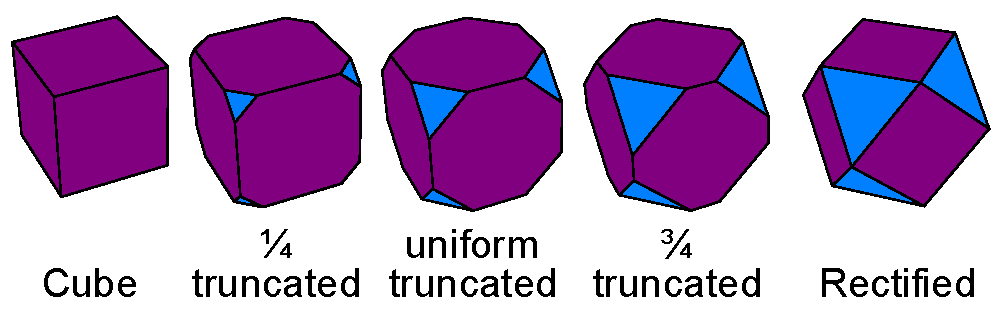
\includegraphics[width=1\textwidth]{../Resources/Figs/truncation.pdf}
        \caption{Trunctation and rectification operations visualised \cite{wikimedia-cube-truncation}}
        \label{fig:truncation}
    \end{figure}
    \item[Expansion/Cantellation] All the facets are pulled out away from the centroid of the polyhedron by the same distance without rescaling. The empty spaces are then filled with regular polygons in the following way: Edges that used to be identical in the original polyhedron are connected by adding a new a square. All the vertices that corresponded to a single vertex $v$ in the original polyhedron are connected by adding a $d$-gon where $d=deg(v)$.

    This operation can also be described as cantellation. The difference is in how we imagine the process that takes us to the resulting shape. From the viewpoint of cantellation, we first bevel (cut off) the edges and then apply truncation on what remained from the original vertices.
        \begin{figure}[H]
        \centering
        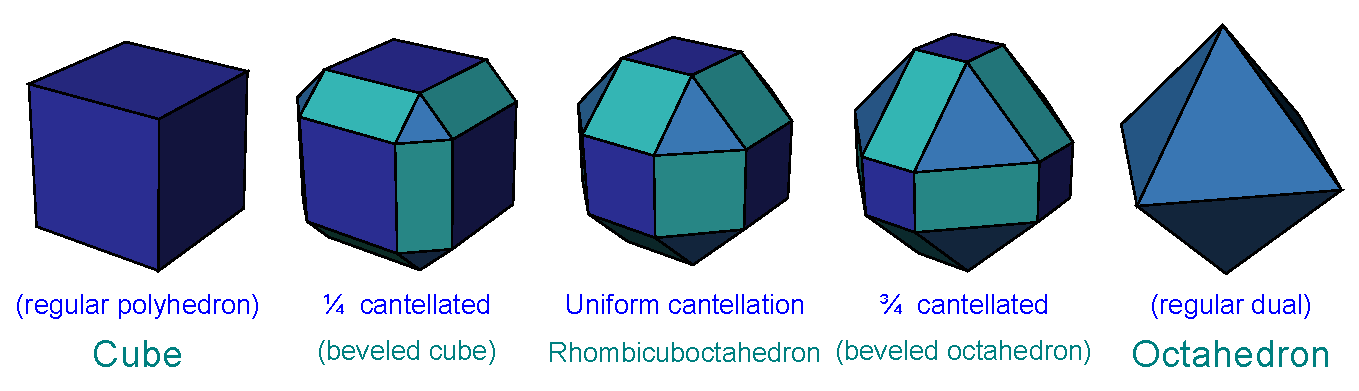
\includegraphics[width=1\textwidth]{../Resources/Figs/cantellation.pdf}
        \caption{Cantellation operation visualised \cite{wikimedia-cube-cantellation}}
        \label{fig:cantellation}
    \end{figure}
    \item[Snub] Is an application of expansion followed by splitting each new square in half in such a way, that we can twist the facets of the original Platonic solid.
\end{description}


\todo{TODO: Add visualisation of snub operation}

\begin{highlight}
\section*{Platonic and Archimedean graph properties}

Here I would like to list some properties, that the graphs corresponding to the solids described above have.

\end{highlight}

\chapter{Definitions}

Since the main concern of this thesis is coloring of the graphs mentioned in the preface, it is useful to define all the necessary concepts we will be working with.

\section{Basic definitions and assumptions}

Here we state mathematical definitions, that should not be surprising in any way. Also, we state some assumption we will make, which will then hold for the rest of this thesis.

\begin{definition}
    An \textit{undirected graph} $G$ is an ordered pair $G=(V,E)$ where $V$ is a set of vertices of the graph and $E \subseteq \binom{V}{2}$ is the set of its edges. 
\end{definition}

\begin{assumption}
    For any graph $G=(V,E)$ we will assume $V \cap E = \emptyset$. 
\end{assumption}

\begin{definition}
    A \textit{partial function} is a function $f:X \rightarrow Y$ s.t. $\forall x \in X$ we have $f(x) \in Y$ or $f(x)$ is undefined.
\end{definition}

\section{General coloring}
\todo[inline]{JF: Co třeba General concept of coloring nebo Common properties of colorings nebo Concept of coloring?

General coloring zní jako byste chtěl studovat to jedno barvení, které se nazývá "obecné barvení"}

As we will be working with many different colorings, to avoid repetition, we will define the notion of an abstract coloring which all the concrete colorings will share.

\todo[inline]{JF: nevím, jestli někdy nebudete chtít barvit i stěny třeba v tzv. perfect coloring.
Pěkný přehled o barveních je zde: \url{https://fs.unm.edu/IJMC/Graph_Coloring,Types_and_Applications_A_Survey.pdf}

Jinak, co přečtu, tomu zakomentuji {\tt $\{$highlight$\}$} OK?
}

\begin{definition}
    For $k \in \mathbb{N}$ and a graph $G=(V,E)$ \textit{coloring} of $G$ is a partial function $c: V \cup E \rightarrow \{1,\ldots,k\}$ with a coloring rule $R$ that restricts, which elements of the graph cannot share the same color.
\end{definition}

\todo[inline]{JF: Zvažte, jestli obecné obarvení neuvést třeba nějak jako:

The concept of coloring is in mathematical sense equivalent to the concept of mapping, when the domain --- the set of colors --- is usually a finite set without any further structure. So the only relevant characteristic is, whether two elements are mapped on the same target, or to phrase less colloquially: colored by the same color.

Hence we may without loss of generality assume that the domain is a set of positive integers, however sometimes we use usual colors like \emph{red}, \emph{blue}, etc, to visualize some particular colorings in more accessible way.
}

In other words, coloring is an assignment of numbers to vertices, edges or both s.t. based on the coloring rule, certain vertices or edges cannot share the same color. The coloring rule is usually independent on the choice of graph.

\begin{definition}
    Let the set of all colorings sharing the same coloring rule $R$ be called a \textit{family of colorings}.
\end{definition}

%\begin{highlight}
\begin{definition}
    Let $G=(V,E)$, let $F$ be a family of colorings, let $k \in \mathbb{N}$. \\ A function $c \in F$ such that $c: V \cup E \rightarrow \{1,\ldots,k\}$ is called a \textit{k-coloring} of $G$.
\end{definition}

Note that a $k$-coloring does not necessarily have to use all of the $k$ available colors. Mathematically speaking, a $k$-coloring is not necesserily a surjective function.

\begin{definition}
    For a graph $G=(V,E)$, family of colorings $F$ and a natural number $k$, if there exists a k-coloring of $G$ then we say that $G$ is \textit{k-colorable}.
\end{definition}

    A typical question we ask ourselves when considering colorings of graph is: What is the least amount of colors we can use to color the graph, without breaking the coloring rule? This leads to a definition of so called \textit{chromatic number}. 
%\end{highlight}

\begin{definition}
    For a graph $G$ and a family of colorings $F$, let \textit{chromatic number} $\chi ^F (G)$ be the minimum $k \in \mathbb{N}$ s.t. $G$ is k-colorable.
\end{definition}

%\begin{highlight}
    Once we know a graph is k-colorable, there is another interesting property of the graph we can examine. We can ask about how many different colorings with k colors there exists for the given graph. A closely related concept to this question is the \textit{chromatic polynomial}.

    \begin{definition}
        Given a graph $G=(V,E)$, family of colorings $F$ and k-colorings $c_1,c_2 \in F$: $c_1$ and $c_2$ are different if there exists $x \in V \cup E$ s.t. $c_1(x) \neq c_2(x)$.
    \end{definition}

    The definition above states, that if two colorings assign some element a different color, then the colorings are considered different. Note that this does not take into account any symmetries of the graph.

    \begin{definition}
        For graph $G$ and a family of colorings $F$, the \textit{chromatic polynomial} denoted by $P^{F}_G(x)$ is a function s.t. $\forall k \in \mathbb{N} : P^{F}_G(k) = n$, where $n$ is the number of different k-colorings of $G$.
    \end{definition}

    For example, given the graph of tetrahedron $K_4$, the chromatic polynomial $P^{F_V}_G(x) = x \cdot (x-1) \cdot (x-2) \cdot (x-3)$. This can be seen if we label the vertices $v_1,v_2,v_3,v_4$ and imagine coloring them sequentially in the order of their labels. We have exactly $x$ colors left to use for the first vertex. With each other vertex, we have one less color available to use. 
    
%\end{highlight}

\section{Specific colorings}

\subsection{Vertex coloring}

\begin{definition}
    A \textit{vertex coloring} of a graph $G=(V,E)$ is a coloring $c : V \rightarrow \mathbb{N}$ belonging to family of colorings with the following coloring rule:
    \begin{equation}\label{eqn:vtx_rule}
        \forall u,v \in V, \quad \text{if } \{u,v\} \in E, \text{ then } c(u) \neq c(v). 
        \tag{$R_V$}
    \end{equation}
    We will denote this family of colorings by $F_V$.
\end{definition}

In other words, vertex coloring is an assignment of colors to each vertex s.t. no two vertices connected by an edge share the same color.

\begin{figure}[H]
    \centering
    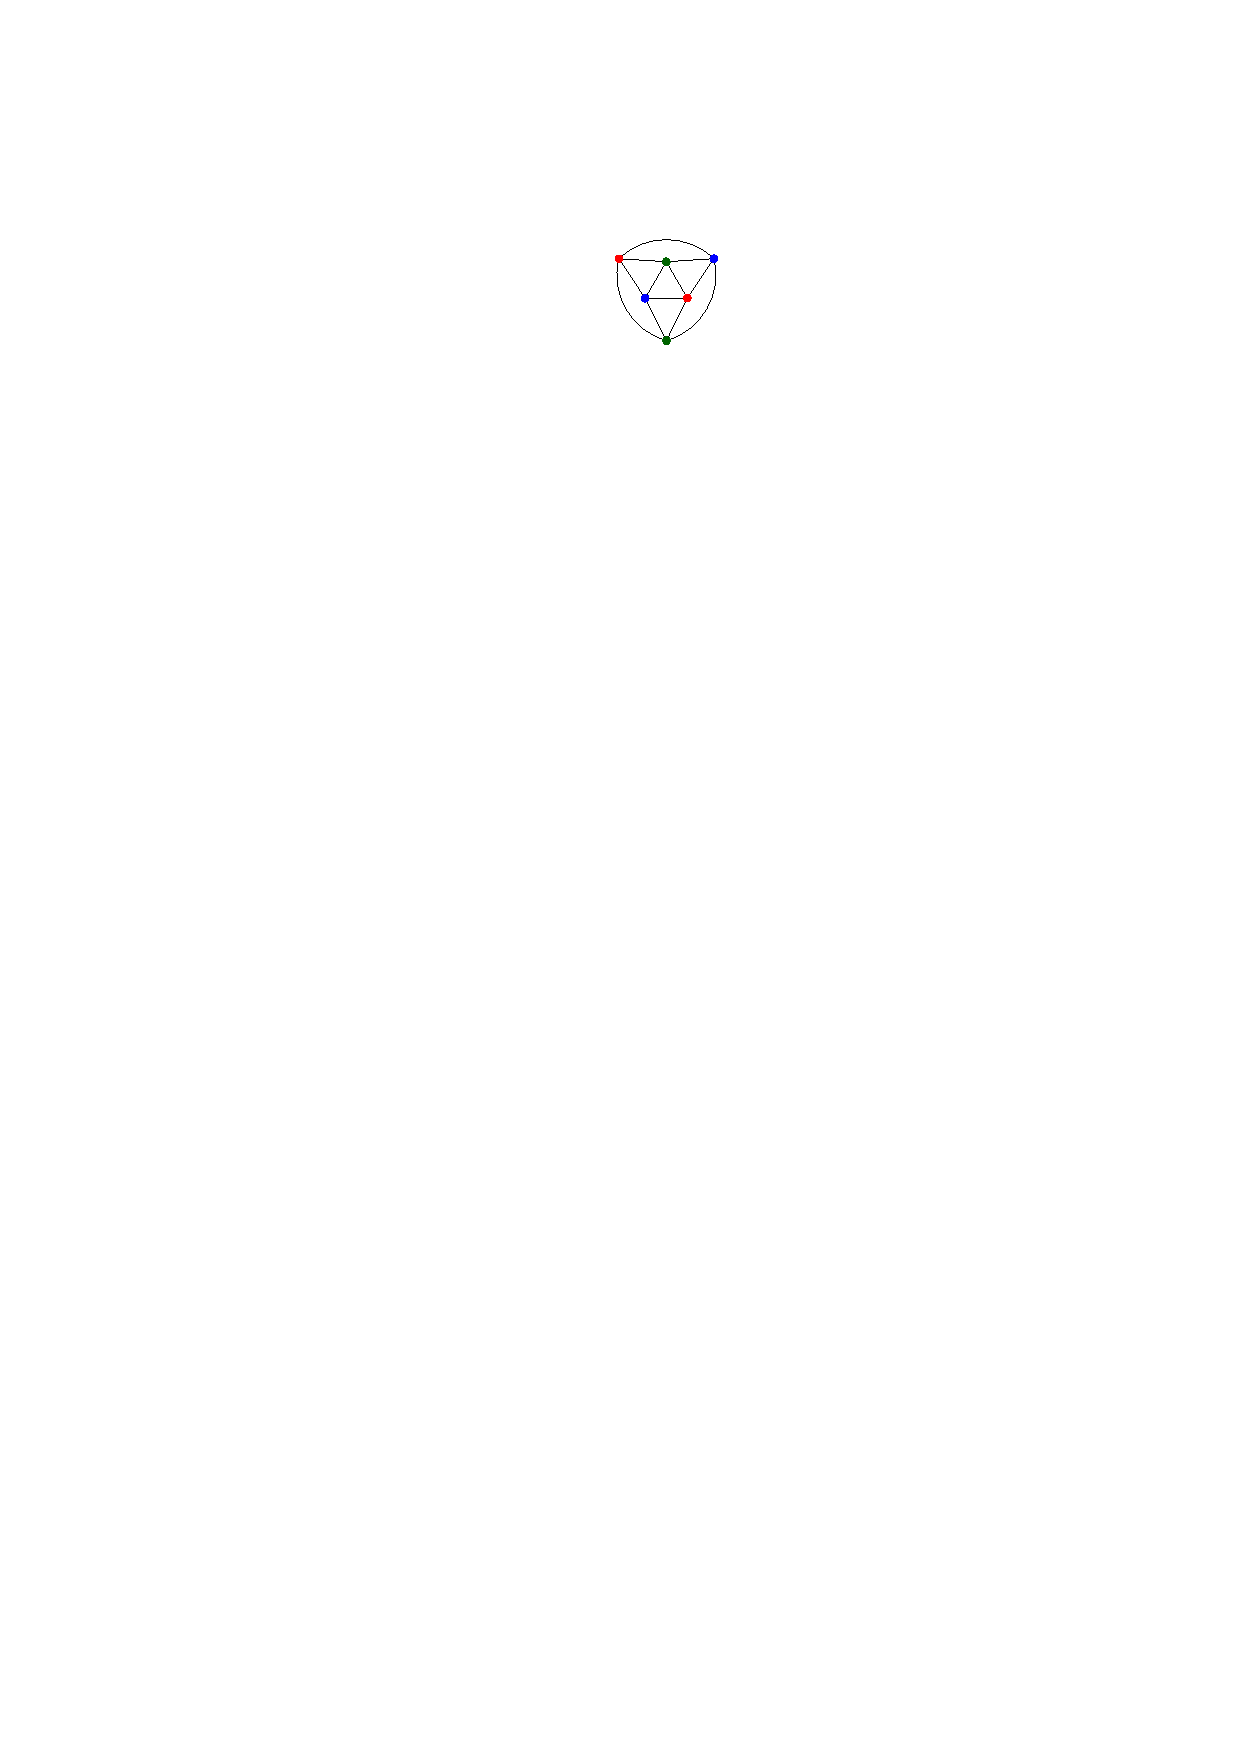
\includegraphics[width=0.2\textwidth]{../Resources/Figs/octahedral_vtx_colr.pdf}
    \caption{Vertex coloring of octahedral graph}
    \label{fig:octahedral_vtx_coloring}
\end{figure}

The graph in figure~\ref{fig:octahedral_vtx_coloring} has vertex chromatic number 3.

\subsection{Edge coloring}

\begin{definition}
    An \textit{edge coloring} of a graph $G=(V,E)$ is a coloring $c: E \rightarrow \mathbb{N}$ belonging to family of colorings for which the coloring rule is: 
    \begin{equation}\label{eqn:edge_rule}
     \forall e,f \in E, \quad \text{ whenever } e \cap f \neq \emptyset \text{ then } c(e) \neq c(f) \tag{$R_E$}
    \end{equation}
    We will denote this family of colorings by $F_E$.
   
\end{definition}

What the definition above says is, that whenever two edges share an endpoint, they cannot share the same color. 

\begin{figure}[H]
    \centering
    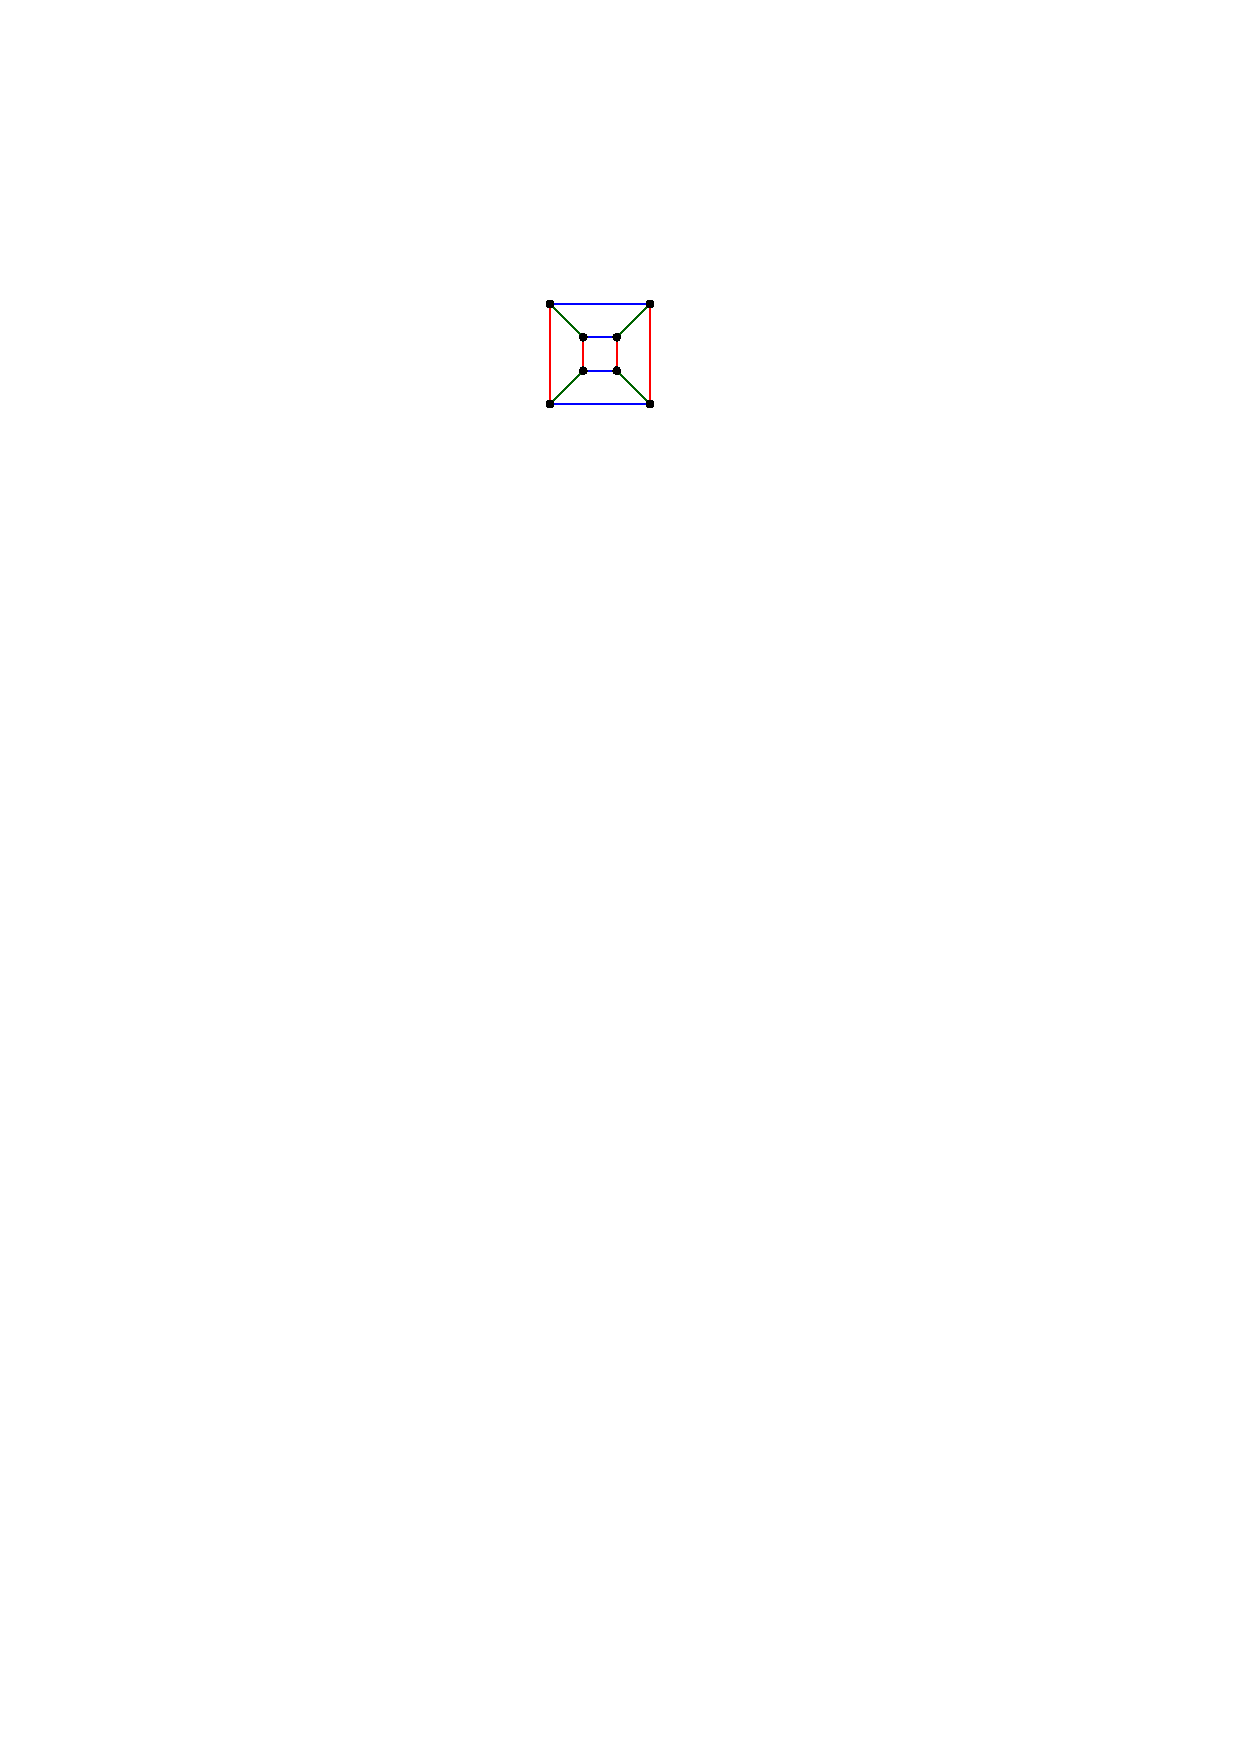
\includegraphics[width=0.2\textwidth]{../Resources/Figs/cubical_edg_colr.pdf}
    \caption{Edge coloring of cubical graph}
    \label{fig:cubical_edge_coloring}
\end{figure}

\subsection{Computed vertex and edge chromatic numbers}

\begin{highlight}
    
The vertex and edge chromatic numbers can be computed in little time using \textit{SageMath} functions \cite{sagemath-chromatic-number} \cite{sagemath-chromatic-index}. The following two tables provide overview of vertex chromatic numbers $\chi(G)$  and edge chromatic numbers $\chi'(G)$ for Platonic and Archimedean solids. Note that the edge chromatic number $\chi'(G)$ is also called the \textit{chromatic index}.
\end{highlight}

\begin{center}
\begin{tabular}{|l|c|c|}
\hline
Platonic & $\chi(G)$ & $\chi'(G)$ \\
\hline\hline
cube & 2 & 3 \\
\hline
dodecahedron & 3 & 3 \\
\hline
icosahedron & 4 & 5 \\
\hline
octahedron & 3 & 4 \\
\hline
tetrahedron & 4 & 3 \\
\hline
\end{tabular}
\end{center}

\begin{center}
\begin{tabular}{|l|c|c|}
\hline
Archimedean & $\chi(G)$ & $\chi'(G)$ \\
\hline\hline
cuboctahedron & 3 & 4 \\
\hline
icosidodecahedron & 3 & 4 \\
\hline
rhombicosidodecahedron & 3 & 4 \\
\hline
rhombicuboctahedron & 3 & 4 \\
\hline
snub cube & 3 & 5 \\
\hline
snub dodecahedron & 4 & 5 \\
\hline
truncated cube & 3 & 3 \\
\hline
truncated cuboctahedron & 2 & 3 \\
\hline
truncated dodecahedron & 3 & 3 \\
\hline
truncated icosahedron & 3 & 3 \\
\hline
truncated icosidodecahedron & 2 & 3 \\
\hline
truncated octahedron & 2 & 3 \\
\hline
truncated tetrahedron & 3 & 3 \\
\hline
\end{tabular}
\end{center}


\subsection{Total coloring}

\begin{definition}
    A \textit{total coloring} of graph $G=(V,E)$ is a coloring $c: V \cup E \rightarrow \mathbb{N}$ from family of colorings sharing both coloring rules \ref{eqn:vtx_rule} and \ref{eqn:edge_rule} and the following additional rule: 
    \begin{equation}\label{eqn:tot_rule}
    \forall v \in V,  \forall e \in E, \text{ if } \{v\} \cap e \neq \emptyset \text{ then } c(v) \neq c(e) \tag{$R_T$}
    \end{equation}
    We will call this family $F_T$.
\end{definition}

\begin{figure}[H]
    \centering
    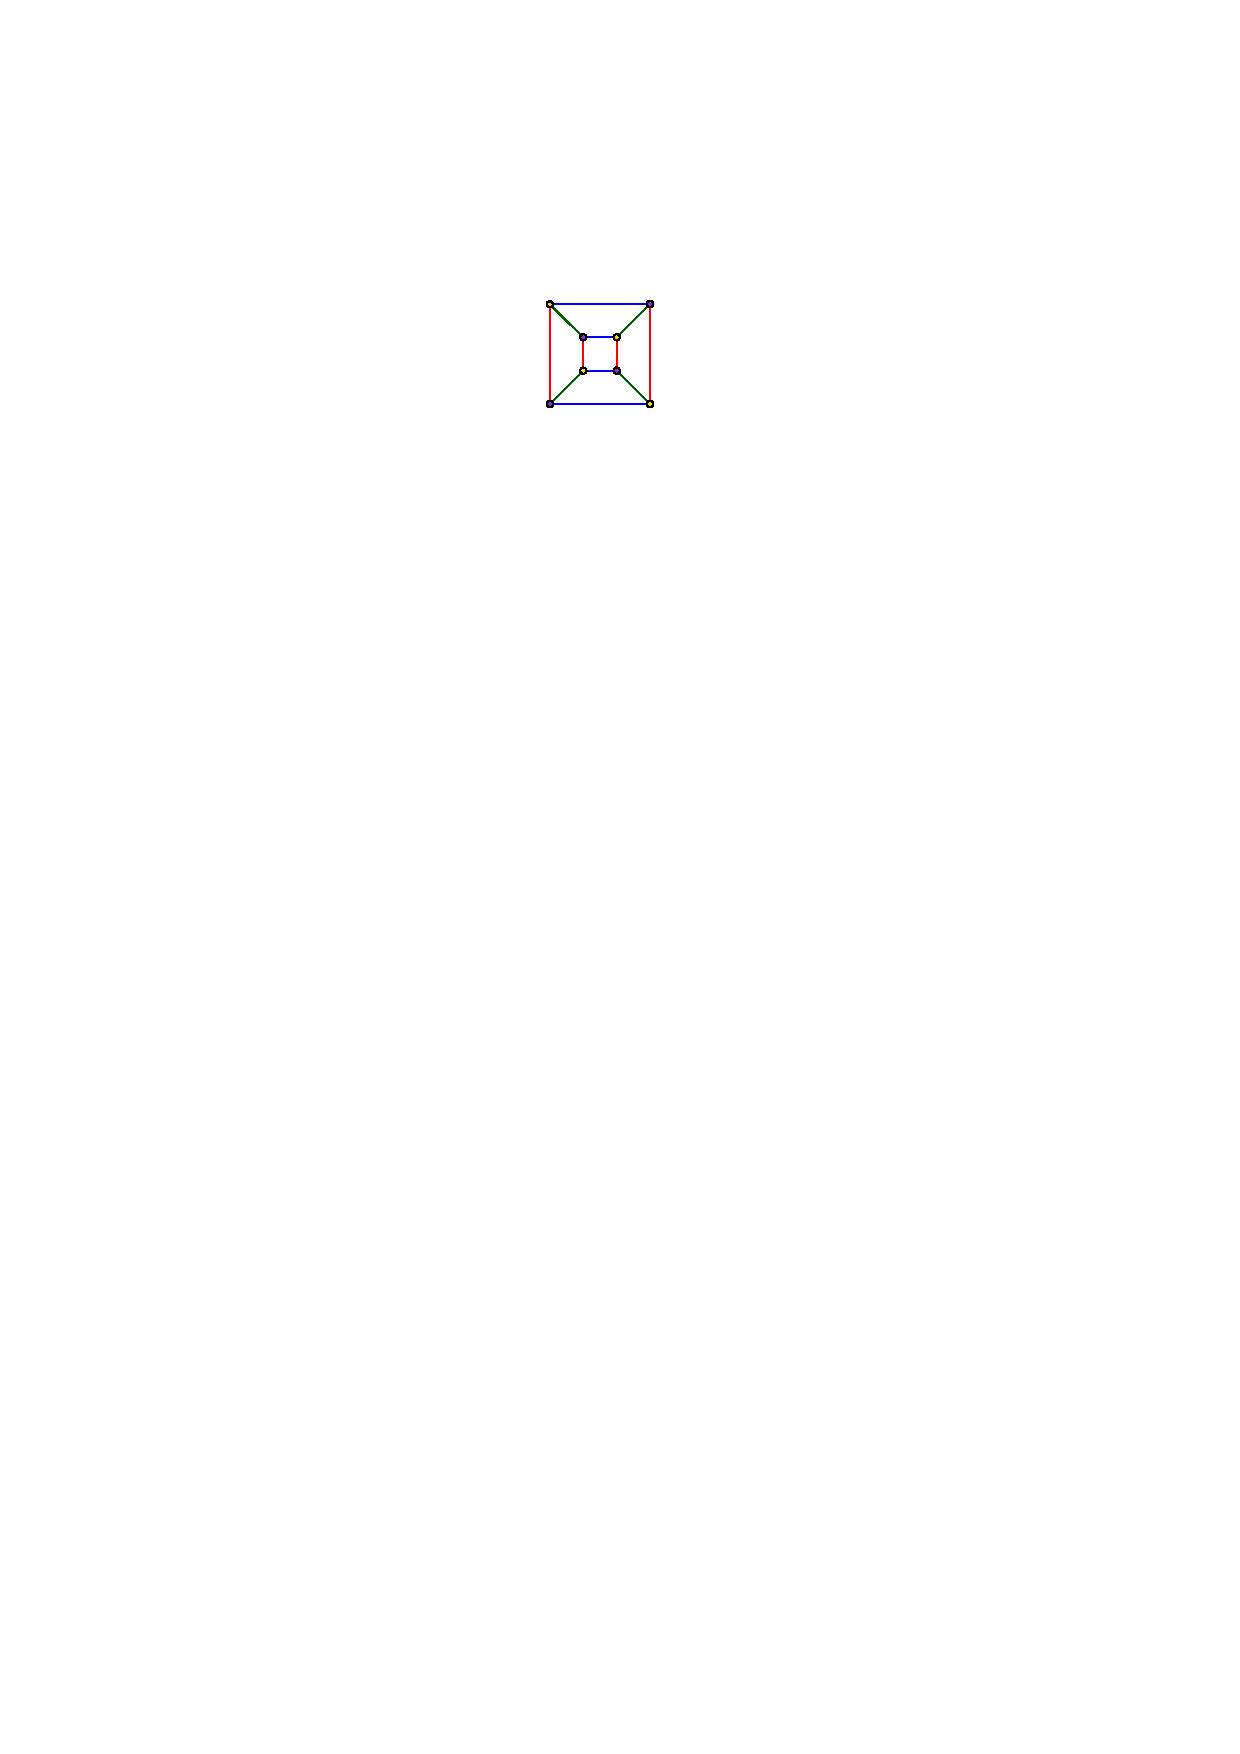
\includegraphics[width=0.2\textwidth]{../Resources/Figs/cubical_tot_colr.pdf}
    \caption{Total coloring of cubical graph using five colors}
    \label{fig:cubical_tot_coloring}
\end{figure}

\begin{figure}[H]
    \centering
    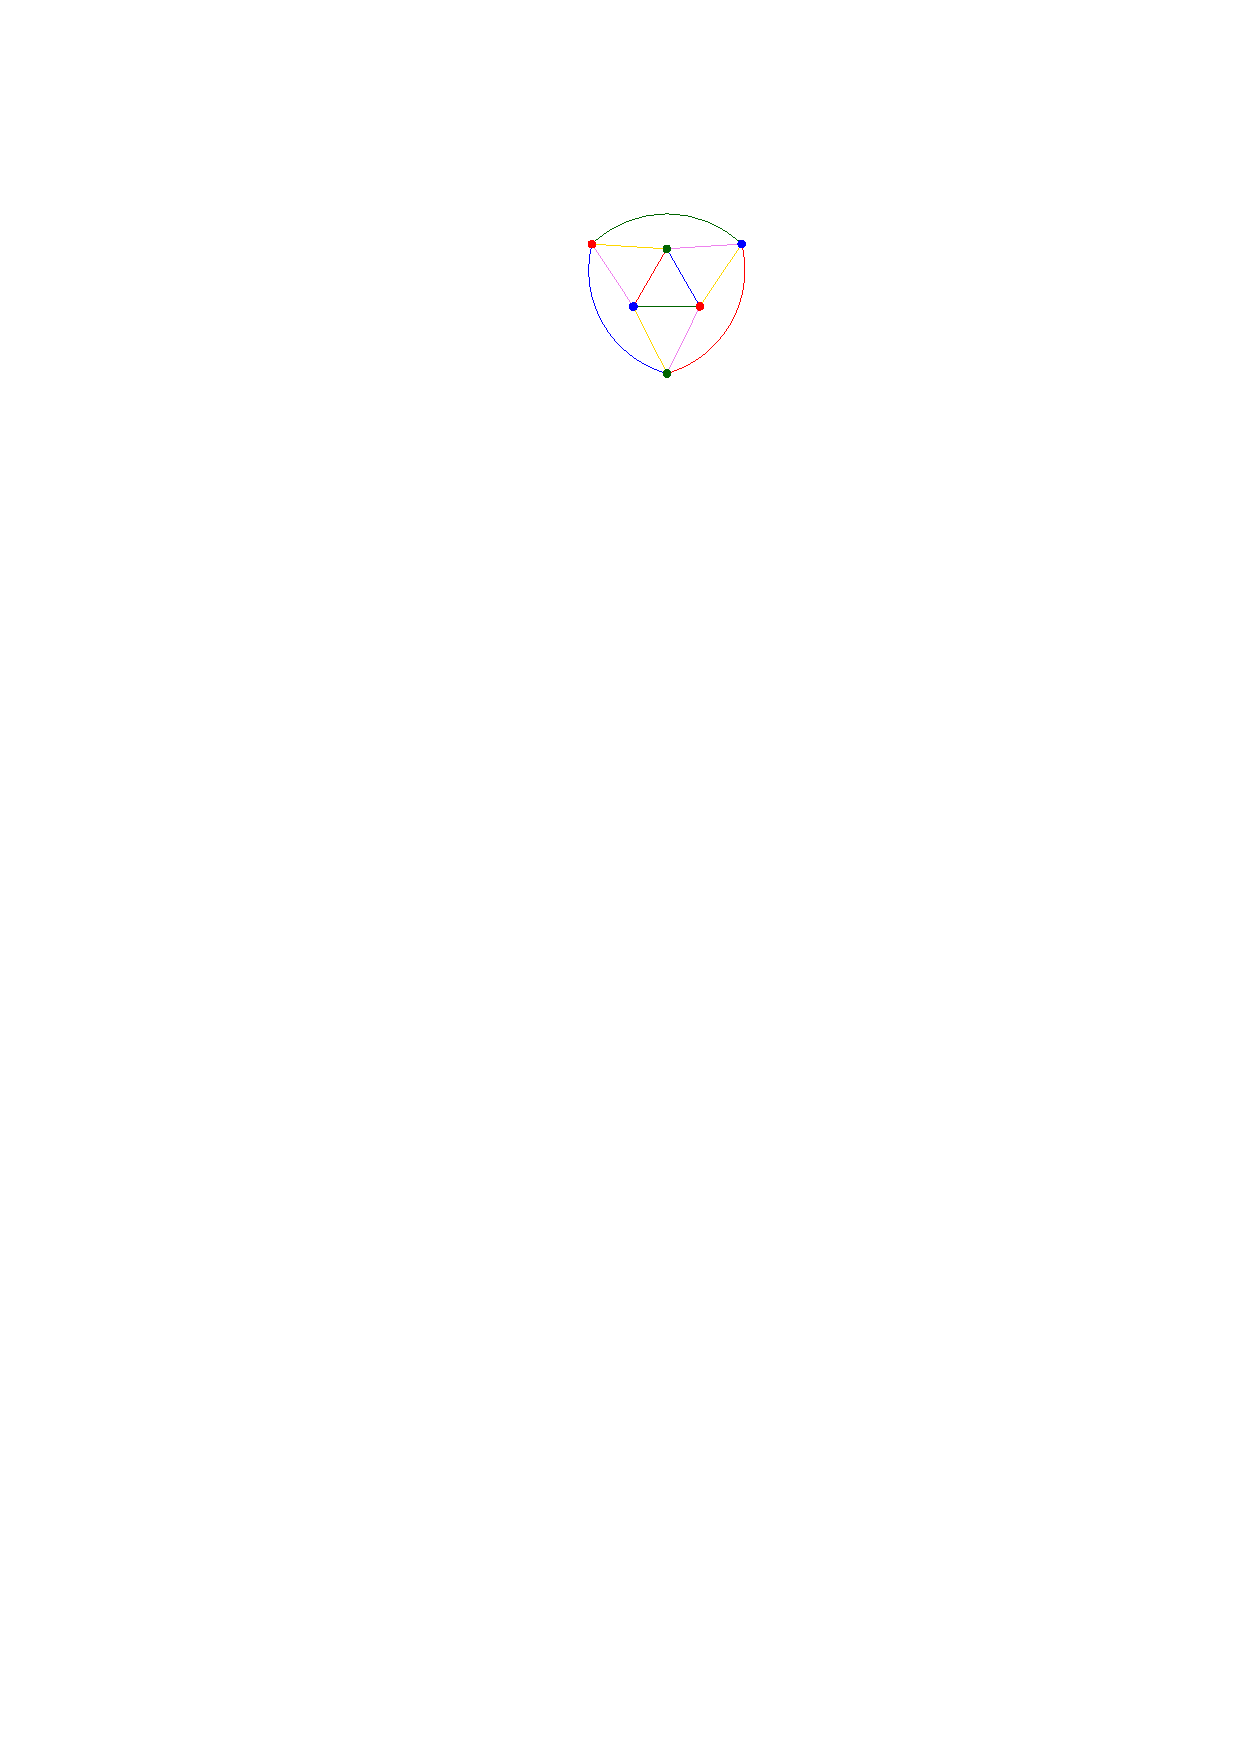
\includegraphics[width=0.2\textwidth]{../Resources/Figs/octahedral_tot_colr.pdf}
    \caption{Total coloring of octahedral graph using five colors}
    \label{fig:octahedral_tot_coloring}
\end{figure}

\todo[inline]{Rainbow coloring a magic labeling -  těmto konceptům se věnovat nejspíš nebudeme, ale bylo by dobré je zmínit někde v úvodu jako barvení, kde jsou ještě další podmínky, resp. kdy hraje roli, jakou hodnotu mají použité barvy.}


\chapter{Colorings considered}

\section{Colorings}

In this chapter I will define 

\section{Title of the second subchapter of the first chapter}


% Ukázka použití některých konstrukcí LateXu (odkomentujte, chcete-li)
%%% Ukázka použití některých konstrukcí LaTeXu

\subsection{Ukázka \LaTeX{}u}
\label{ssec:ukazka}

This short subsection serves as an~example of basic \LaTeX{} constructs,
which can be useful for writing a~thesis.

Let us start with lists:

\begin{itemize}
\item The logo of Matfyz is displayed in figure~\ref{fig:mff}.
\item This is subsection~\ref{ssec:ukazka}.
\end{itemize}

Different kinds of dashes:
red-black (short),
pages 16--22 (middle),
$45-44$ (minus),
and this is --- as you could have expected --- a~sentence-level dash,
which is the longest.
(Note that we have follwed \verb|a| by a~tilde instead of a~space
to avoid line breaks at that place.)

\newtheorem{theorem}{Theorem}
% \newtheorem*{define}{Definition}	% Definice nečíslujeme, proto "*"

\begin{definition}
A~\textit{tree} is a connected graph with no cycles.
\end{definition}

\begin{theorem}
This theorem is false.
\end{theorem}

\begin{proof}
False theorems do not have proofs.
\end{proof}

\begin{figure}
	\centering
	
\includegraphics[width=30mm]{../Resources/Figs/logo.eps}
	\caption{Logo of MFF UK}
	\label{fig:mff}
\end{figure}


\chapter*{Conclusion}
\addcontentsline{toc}{chapter}{Conclusion}


%%% Seznam použité literatury
%%% Seznam použité literatury je zpracován podle platných standardů. Povinnou citační
%%% normou pro bakalářskou práci je ISO 690. Jména časopisů lze uvádět zkráceně, ale jen
%%% v kodifikované podobě. Všechny použité zdroje a prameny musí být řádně citovány.

\def\bibname{Bibliography}
\begin{thebibliography}{99}
\addcontentsline{toc}{chapter}{\bibname}

\bibitem{lamport94}
  {\sc Lamport,} Leslie.
  \emph{\LaTeX: A Document Preparation System}.
  2. vydání.
  Massachusetts: Addison Wesley, 1994.
  ISBN 0-201-52983-1.

\end{thebibliography}


%%% Tabulky v bakalářské práci, existují-li.
\chapwithtoc{List of Tables}

%%% Použité zkratky v bakalářské práci, existují-li, včetně jejich vysvětlení.
\chapwithtoc{List of Abbreviations}

%%% Přílohy k bakalářské práci, existují-li (různé dodatky jako výpisy programů,
%%% diagramy apod.). Každá příloha musí být alespoň jednou odkazována z vlastního
%%% textu práce. Přílohy se číslují.
\chapwithtoc{Attachments}

\openright
\end{document}
